\section{Discussion}\label{sec:discussion}

\paragraph{What test signatures can and cannot tell an instructor}
The classic pipeline---test-case OAV, K-means or Hamming clustering, induced IF--THEN rules---recovers the most frequent failure of this course well: output-text errors produce distinctive signatures, and on real repairs the signature clusters reach a moderate ARI of {{real_ari_outcomes}}. But the representation cannot separate mechanisms that fail the same tests. On controlled mutants of the same programs, where every mechanism is present, its clusters barely agree with mechanisms (ARI {{injected_ari_outcomes}}), and even a perfect classifier reading only the signature could assign at most {{injected_H1a_pct}}\% of items correctly. A dashboard built on signatures therefore reports the common, often specification-level failures accurately and merges the less frequent conceptual ones---wrong branch conditions, missing steps, output format---that are arguably the reason to cluster in the first place.

\paragraph{Output evidence is the cheapest improvement, not new models}
Everything that improved mechanism recovery was already in the autograder's output: relations between actual and expected output and, in our deviation OAV, the kind of numeric and textual deviation. On controlled data this more than tripled the ARI at the same clustering budget, and on real repairs it lifted per-category recovery of the minority mechanisms. Our richer descriptors did not beat simple output relations for clustering (H3), so we do not claim a better clustering method. Their value lies elsewhere: they are problem-agnostic, so rules learned on some assignments apply to others. Rules over aggregated deviation descriptors kept a macro-F1 of {{injected_unseen_problems_evidence_ila2_macro_f1}} on unseen assignments of the controlled benchmark, where rules over outcome summaries were near zero; per-test signatures cannot even be compared across assignments.

\paragraph{Rules as checked hypotheses}
ILA and ILA-2 produce the production rules that the classic formulation asks for, and ILA-2's penalty trades a small loss of precision for much larger coverage. A shallow CART tree over the same attributes is about as accurate, so the case for ILA-2 is not accuracy but form: an ordered list of short IF--THEN rules, each with a support count, that an instructor can read and falsify, and that abstains instead of guessing when no rule matches. On real repairs the advantage of evidence rules over outcome-summary rules was not statistically reliable with the {{real_seen_problems_evidence_ila2_n}} sealed test items, so these rules should be read as starting points for an instructor's judgement, not as diagnoses.

\paragraph{Embeddings find authors before mechanisms}
A strong general-purpose code embedding grouped mutants by the program they came from: one-token changes that decide behaviour barely move the vector, while identifiers, layout and solution strategy dominate it. This does not contradict earlier successes with embeddings trained on the task \citep{shi2021misconception,piech2015embeddings}; it shows that a frozen embedding needs execution evidence or mechanism-aware training before its clusters can be read as error groups.

\subsection{Implications for instructors and tool builders}\label{sec:tool}
We turned these findings into a local instructor tool, AAI Lab (\cref{fig:tool}), whose design follows from the evidence rather than from the classic formulation. For every exercise, the latest failing submission of each learner is represented with the registered deviation OAV and clustered with K-means, with $k$ chosen by silhouette unless the instructor sets it. Each group shows (i) its test signature and, for every test, the failure rate of the group next to that of the other groups, (ii) the output deviations shared by at least 60\% of its members, and (iii) one IF--THEN rule induced by ILA-2 on the class itself, reported with its precision and coverage. A mechanism hypothesis is stated only when one rule covers at least half of the group: either a hand-written rule for that exercise or for C programs in general, or one of the {{n_frozen_rules}} ILA-2 rules learned from real repairs and frozen before deployment. Otherwise the group is labelled as having no hypothesis, and when its members match different rules the tool says so explicitly, as for the programs of \cref{fig:example}. Every hypothesis comes with one question to ask students and one re-teaching activity, and the instructor confirms or rejects the group; programs run only in an isolated container, and the tool serves the local machine only.

Three lessons from the study shaped this design. First, a group is described by what its members share, never by the signature alone, because RQ1 showed that signatures merge mechanisms. Second, the tool abstains and flags mixed groups rather than naming every cluster, because RQ3 showed that even the best rules leave many items unexplained on real data. Third, mechanism hypotheses are phrased as questions to check with students, because a repair-grounded label describes a program change, not a belief. We have not yet evaluated the tool with instructors; whether its groups and hypotheses change teaching decisions is an open question for a classroom study.

\begin{figure}[!tbp]
\centering
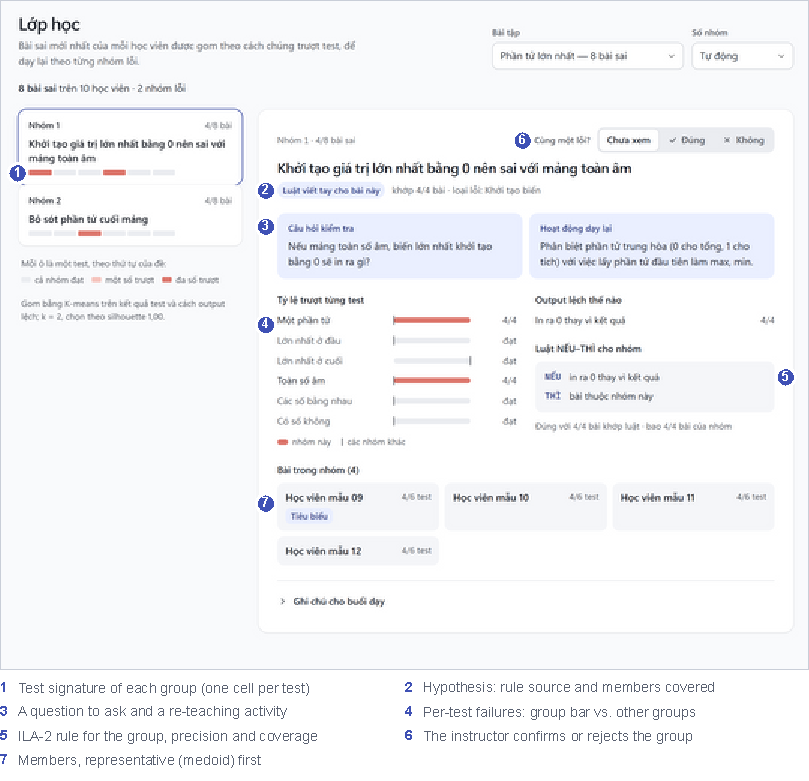
\includegraphics[width=\textwidth]{figures/fig8_tool_en.pdf}
\caption{The class view of AAI Lab for one exercise of a demonstration class written by the authors (interface in Vietnamese). The selected group of four submissions fails the tests with a single element and with only negative numbers; the hand-written exercise rule ``largest value initialised to 0'' covers all four, and the rule induced on the class reads ``IF the output is 0 instead of the result''.}\label{fig:tool}
\end{figure}

\subsection{Repair-grounded evaluation}
Verified minimal repairs turned {{n_pairs}} naturally occurring repair events into auditable labels at the cost of {{probes_total}} program executions and no annotation hours. Two findings matter beyond this study. First, {{multi_share}}\% of minimal repairs changed more than one kind of code, so partitioning failed submissions into single-mechanism clusters is itself a simplification; overlapping or multi-label grouping deserves more attention. Second, a controlled benchmark built with the same taxonomy exposes limits that the imbalanced real distribution hides, and the two benchmarks disagree exactly where the dominant real category is easy.

%%INCLUDE sections/limitations.tex
